\section{Ray Tracing}
\label{sec:chapter_stato_arte_ray_tracing}

In computer grafica, ray tracing è una tecnica di rendering che permette di generare un’ immagine tracciando la direzione della luce attraverso ogni pixel della scena da renderizzare.
Essa viene utilizzata per determinare quali oggetti sono visibili dall’ osservatore, ovvero la camera, e quali di questi sono illuminati o in ombra.
Il meccanismo base è semplice, vengono lanciati dei raggi (view ray) da ogni pixel del piano immagine, che rappresenta l’immagine a due dimensioni dell’ ambiente osservato dalla camera, verso la scena. 
Per ogni raggio lanciato viene calcolato l’oggetto più vicino a partire dall’ osservatore. Dall’oggetto viene lanciato un nuovo raggio (shadow ray) verso ogni luce e viene valutata la presenza di un altro oggetto tra i due.
Se tale oggetto è presente ed è opaco, allora la luce viene bloccata, se invece è trasparente la luce viene attenuata.
Se tale oggetto è assente allora l’ oggetto intersecato dal primo raggio viene colpito dalla luce.
Quindi il colore di uno specifico pixel da mostrare sul piano immagine viene calcolato in base al colore ed alle proprietà del materiale del primo oggetto intersecato dal view ray, insieme alla quantità di luce che quel pixel riceve dalle luci presenti nella scena, calcolate grazie agli shadow ray.
\\
\begin{figure}[htb]
 \centering
 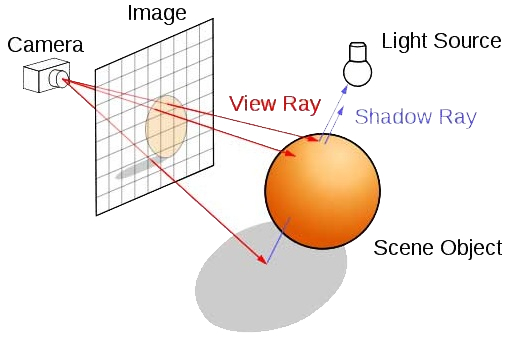
\includegraphics[width=0.8\linewidth]{images/chapter_stato_arte/stato_arte_raytracing_shadowray.jpg}\hfill
 \caption[Ray tracing e shadow ray]{Algoritmo di ray tracing, ed utilizzo dello shadow ray}
 \label{fig:stato_arte_raytracing_shadowray}
\end{figure}

Altri raggi possono essere lanciati dall’ oggetto intersecato dal view ray in maniera tale da consentire la crazione di un’effetto di riflessione e/o rifrazione.
Se l’ oggetto intersecato è ad esempio riflettente, un raggio può essere generato verso la direzione di riflessione.
Questo raggio prende il colore del primo oggetto intersecato. Dal punto appena intersecato viene nuovamente lanciato il ray shadow insieme ad un’ulteriore raggio nella direzione di riflessione e/o rifrazione, a seconda del fenomeno provocato dall’oggetto colpito. Questo procedimento viene ripetuto ricorsivamente fino a quando una superficie non riflettente viene colpita o fino quando il contributo massimo di rimbalzi non viene raggiunto.
Se l’ oggetto intersecato è solido e trasparente, un nuovo raggio può essere generato nella direzione di rifrazione, ed esattamente come per la riflessione questo verrà valutato ricorsivamente.
\\
\begin{figure}[htb]
 \centering
 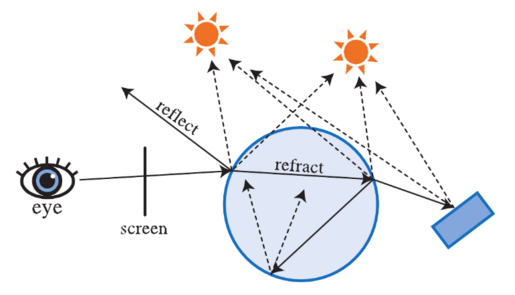
\includegraphics[width=0.8\linewidth]{images/chapter_stato_arte/stato_arte_refr_refl.png}\hfill
 \caption[Ray tracing ed effetti di rifrazione/riflessione]{Algoritmo di ray tracing e gestione degli effetti di rifrazione e riflessione}
 \label{fig:stato_arte_refr_refl}
\end{figure}

Il problema principale è il fatto che, oltre alle sorgenti luce, ogni singolo oggetto visibile ad occhio nudo riflette luce ed il ray tracing calcola solamente le luci dirette alle superfici mentre quelle indirette vengono completamente ignorate. L’ algoritmo di path tracing risolve questa limitazione.